% To be compiled by XeLaTeX, preferably under TeX Live.
% LaTeX source for ``Yanqi Lake Lectures on Algebra'' Part III.
% Copyright 2019  李文威 (Wen-Wei Li).
% Permission is granted to copy, distribute and/or modify this
% document under the terms of the Creative Commons
% Attribution-NonCommercial 4.0 International (CC BY-NC 4.0)
% https://creativecommons.org/licenses/by-nc/4.0/

% To be included
\chapter{Dimension of finitely generated algebras}

The main reference is \cite[\S 13]{Mat80}.

\section{Dimensions in fibers}
Consider a homomorphism $\varphi: A \to B$, which induces $\varphi^\sharp: \Spec(B) \to \Spec(A)$ on prime spectra. Given $\mathfrak{p} \in \Spec(A)$, we are interested in the fiber $(\varphi^\sharp)^{-1}(\mathfrak{p})$; the prime ideals $\mathfrak{q}$ therein are described by $\varphi^{-1}(\mathfrak{q}) = \mathfrak{p}$, or equivalently:
\[ \varphi^{-1}(\mathfrak{q}) \cap (A \smallsetminus \mathfrak{p}) = \emptyset, \quad \mathfrak{q} \supset \varphi(\mathfrak{p}). \]
Adopt the convention that a zero ring has $\Spec = \emptyset$. The first condition says that $\mathfrak{q}$ comes from $\Spec(B_{\mathfrak{p}})$, where $B_{\mathfrak{p}}$ is the localization with respect to $\varphi(A \smallsetminus \mathfrak{p})$ (possibly zero). The second condition then says that $\mathfrak{q}B_{\mathfrak{p}}$ lies over the image of $\mathfrak{p}A_{\mathfrak{p}}$. Set
\[ \kappa(\mathfrak{p}) := A_{\mathfrak{p}}/\mathfrak{p}A_{\mathfrak{p}}. \]
The fiber $(\varphi^\sharp)^{-1}(\mathfrak{p})$ is then identified with the spectrum of
\[ B \dotimes{A} \kappa(\mathfrak{p}) = \left( B \dotimes{A} A_{\mathfrak{p}} \right) \dotimes{A_{\mathfrak{p}}} \kappa(\mathfrak{p}) = B_{\mathfrak{p}} \dotimes{A_{\mathfrak{p}}} (A_{\mathfrak{p}}/\mathfrak{p}A_{\mathfrak{p}} ), \]
which is empty if and only if $B \dotimes{A} \kappa(\mathfrak{p})$ is zero. This also equips $(\varphi^\sharp)^{-1}(\mathfrak{p})$ with an extra structure: it is the spectrum of an explicit quotient ring of $B_{\mathfrak{p}}$.

Observe that for all $\mathfrak{q} \in (\varphi^\sharp)^{-1}(\mathfrak{p})$, the localization of $B_{\mathfrak{p}} \dotimes{A_{\mathfrak{p}}} \kappa(\mathfrak{p})$ at the image of $\mathfrak{q}$ is canonically isomorphic to $B_{\mathfrak{q}} \dotimes{A_{\mathfrak{p}}} \kappa(\mathfrak{p})$.

\begin{proposition}\label{prop:fiber-ineq}
	Assume $A, B$ to be Noetherian. Let $\mathfrak{q} \in \Spec(B)$ and $\mathfrak{p} := \varphi^\sharp(\mathfrak{q})$. We have
	\begin{enumerate}[(i)]
		\item $\dim(B_{\mathfrak{q}}) \leq \dim(A_{\mathfrak{p}}) + \dim B_{\mathfrak{q}} \dotimes{A_{\mathfrak{p}}} \kappa(\mathfrak{p})$ (note that the existence of $\mathfrak{q}$ ensures that $B_{\mathfrak{p}} \dotimes{A_{\mathfrak{p}}} \kappa(\mathfrak{p}) \neq \{0\}$, hence $B_{\mathfrak{q}} \dotimes{A_{\mathfrak{p}}} \kappa(\mathfrak{p}) \neq \{0\}$);
		\item equality holds if going-down holds for $\varphi$;
		\item if going-down holds and $\varphi^\sharp$ is surjective, then $\dim(B) \geq \dim(A)$, and for all ideal $\mathfrak{a} \subsetneq A$ we have $\varphi(\mathfrak{a}) B \neq B$ and $\mathrm{ht}(\mathfrak{a}) = \mathrm{ht}(\varphi(\mathfrak{a})B)$.
	\end{enumerate}
\end{proposition}

It is crucial to notice that $\dim B_{\mathfrak{q}} \dotimes{A_{\mathfrak{p}}} \kappa(\mathfrak{p}) = \text{ht}(\mathfrak{q}B_{\mathfrak{q}}/\varphi(\mathfrak{p}) B_{\mathfrak{q}}) = \text{ht}(\mathfrak{q}/\varphi(\mathfrak{p})B)$.

This bounds the source dimension of a morphism by the target dimension plus the fiber dimension, localized both at $\mathfrak{p}$ and $\mathfrak{q} \in (\varphi^\sharp)^{-1}(\mathfrak{p})$. In order to have an equality, a certain submersion-like condition on $\varphi^\sharp$ is evidently required; this explains the going-down condition. Cf. \cite[(6.H)]{Mat80}.

\begin{proof}
	We have an induced local homomorphism $A_{\mathfrak{p}} \to B_{\mathfrak{q}}$ since $\mathfrak{q} \mapsto \mathfrak{p}$. Since (i) and (ii) depend only on this induced homomorphism, we may assume from the outset that $A$, $B$ are local with maximal ideals $\mathfrak{p}, \mathfrak{q}$, and $\varphi$ is a local homomorphism. Let $d := \dim A$ and take a parameter ideal $I = (t_1, \ldots, t_d)$ of $A$, so that $\mathfrak{p}^k \subset I \subset \mathfrak{p}$ for some $k$. It follows that $\sqrt{\varphi(\mathfrak{p}) B} = \sqrt{\varphi(I)B}$, therefore $\dim(B \dotimes{A} \kappa(\mathfrak{p})) = \dim(B/\varphi(\mathfrak{p})B) = \dim (B/\varphi(I)B)$; denote this number as $e$. Take a $s_1, \ldots, s_e \in \mathfrak{q}$ whose images generate a parameter ideal for $B/\varphi(I)B$, and put $J := (\varphi(t_1), \ldots, \varphi(t_d), s_1, \ldots, s_e)$. Then $B/J$ is Artinian, therefore $\dim B \leq d+e$ establishes (i).
	
	As for (ii), we conserve the same hypotheses and take a prime chain $\mathfrak{q} = \mathfrak{q}_0 \supsetneq \cdots \supsetneq \mathfrak{q}_e$ with $\mathfrak{q}_e \supset \varphi(\mathfrak{p})B$ in $B$, as well as a prime chain $\mathfrak{p} = \mathfrak{p}_0 \supsetneq \cdots \supsetneq \mathfrak{p}_d$ in $A$. Note that $\varphi^{-1}(\mathfrak{q}_e) = \mathfrak{p}$ since $e = \dim B/\varphi(\mathfrak{p})B$. By applying going-down repeatedly to the chain $\mathfrak{p}_i$, we obtain a prime chain in $B$
	\[ \mathfrak{q}_e \supsetneq \cdots \supsetneq \mathfrak{q}_{e+d}, \quad \varphi^{-1}(\mathfrak{q}_{e+i}) = \mathfrak{p}_i. \]
	Concatenation with $\mathfrak{q}_0 \supsetneq \cdots$ gives $\dim(B) = d + e$. This shows (ii).
	
	The first assertion of (iii) results from (ii). To show the remaining one, let us show $\varphi(\mathfrak{a})B \neq B$: if $\varphi^\sharp(\mathfrak{q}) = \mathfrak{p} \supset \mathfrak{a}$, then $\mathfrak{q} \supset \varphi(\mathfrak{a}) B$. Next, take a minimal over-prime $\mathfrak{q} \supset \varphi(\mathfrak{a})B$ with $\text{ht}(\mathfrak{q}) = \text{ht}(\varphi(\mathfrak{a})B)$. With $\mathfrak{p} := \varphi^{-1}(\mathfrak{q}) \supset \mathfrak{a}$, we must have $\dim B_{\mathfrak{q}} \otimes \kappa(\mathfrak{p}) = \text{ht}(\mathfrak{q}/\varphi(\mathfrak{p})B) = 0$ by the minimality of $\mathfrak{q}$. An application of (ii) yields
	\begin{gather*}
		\text{ht}(\varphi(\mathfrak{a})B) = \text{ht}(\mathfrak{q}) = \text{ht}(\mathfrak{p}) \geq \text{ht}(\mathfrak{a}).
	\end{gather*}
	To obtain $\leq$, choose $\mathfrak{p} \supset \mathfrak{a}$ with $\text{ht}(\mathfrak{p}) = \text{ht}(\mathfrak{a})$ and take $\mathfrak{q} \in \Spec(B)$ with $\mathfrak{p} = \varphi^{-1}(\mathfrak{q})$; this implies $\mathfrak{q} \supset \varphi(\mathfrak{p})B \supset \varphi(\mathfrak{a})B$. Upon shrinking $\mathfrak{q}$, we may even assume $\mathfrak{q}$ is minimal over $\varphi(\mathfrak{p})B$, i.e. $\text{ht}(\mathfrak{q}/ \varphi(\mathfrak{p})B) = 0$. Using (ii), this entails $\text{ht}(\mathfrak{a}) = \text{ht}(\mathfrak{p}) = \text{ht}(\mathfrak{q}) \geq \text{ht}(\varphi(\mathfrak{a})B)$.
\end{proof}

\vspace{1em}
\begin{center}
	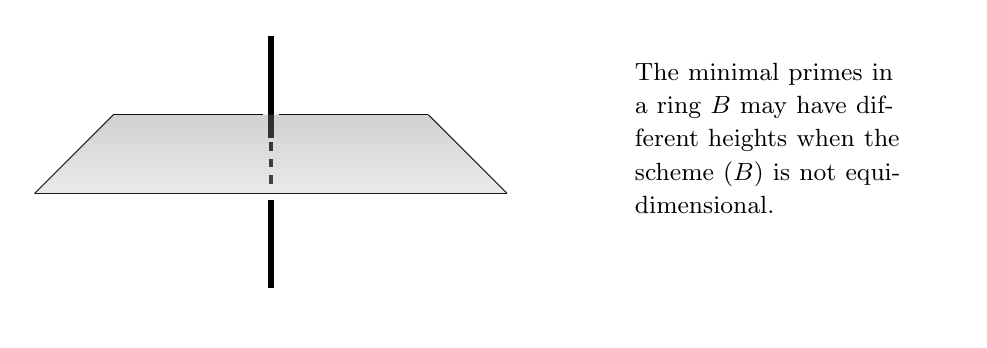
\begin{tikzpicture}
		\draw (-2,1) -- (2,1);
		\draw[line width=6pt, white] (0, 2) -- (0, -1.5);
		\draw[line width=2pt, black] (0,2) -- (0, 0.7);
		\draw[line width=1.5pt, dashed] (0, 0.65) -- (0, 0);
		\draw[line width=2pt, black] (0,0) -- (0, -1.2);
		\draw[line width=5pt, white] (-3,0) -- (3,0);
		\draw (-3,0) -- (3,0);
		\draw (-3,0) -- (-2,1);
		\draw (3,0) -- (2,1);
		\fill[opacity=0.2, shade, color=black!50!white] (-2,1) -- (2,1) -- (3,0) -- (-3,0) -- (-2,1);
		\node[anchor=west, text width=4cm, align=left] at (4.5, 0.7) {\small The minimal primes in a ring $B$ may have different heights when the scheme $\Spec(B)$ is not equi-dimensional.};
	\end{tikzpicture}
\end{center}
\vspace{1em}

Going-down holds for flat $\varphi$ by Theorem \ref{prop:going-down-flat}, therefore the dimension equality
\[ \dim(B_{\mathfrak{q}}) = \dim(A_{\mathfrak{p}}) + \dim B_{\mathfrak{q}} \dotimes{A_{\mathfrak{p}}} \kappa(\mathfrak{p}) \]
holds for flat ring homomorphisms.

\begin{remark}
	In general, if $B$ is a finitely generated algebra over Noetherian $A$ such that $\Spec(B) \to \Spec(A)$ is a closed map, the fiber dimension $\mathfrak{p} \mapsto \dim B/\mathfrak{p}B$ is an \emph{upper semi-continuous function} on the target space $\Spec(A)$. More concretely, the fiber dimension is non-decreasing under specialization of $\mathfrak{p}$. Cf. \cite[\S 14.3]{Eis95} or \cite[(13.E)]{Mat80}. Try to understand this phenomenon intuitively.
\end{remark}

\begin{proposition}\label{prop:dim-integral}
	Suppose $B$ is integral over a subring $A$.
	\begin{enumerate}[(i)]
		\item We have $\dim A = \dim B$.
		\item If we assume moreover that $A, B$ are both Noetherian, then $\mathrm{ht}(\mathfrak{q}) \leq \mathrm{ht}(\mathfrak{q} \cap A)$ for every $\mathfrak{q} \in \Spec(B)$.
		\item Furthermore, if going-down also holds for $A \hookrightarrow B$, we have $\mathrm{ht}(J) = \mathrm{ht}(J \cap A)$ for every ideal $J \subsetneq B$.
	\end{enumerate}
\end{proposition}
\begin{proof}
	Going-up holds and $\Spec(B) \twoheadrightarrow \Spec(A)$ in the situation of (i) by Theorem \ref{prop:Cohen-Seidenberg}, hence $\dim B \geq \dim A$ by lifting prime chains. To prove $\leq$, observe that $\mathfrak{q} \subsetneq \mathfrak{q}'$ implies $\mathfrak{q} \cap A \subsetneq \mathfrak{q}' \cap A$ since there are no inclusion relations in the fibers of $\Spec(B) \to \Spec(A)$.

	As for (ii), note that $\text{ht}(\mathfrak{q}) \leq \text{ht}(\mathfrak{p}) + \text{ht}(\mathfrak{q}/\mathfrak{p}B)$ where $\mathfrak{p} := \mathfrak{q} \cap A$; as the are no inclusion relations in fibers, the last term must be $0$.
	
	Now assume going-down and consider (iii). Take $\mathfrak{q} \in \Spec(B)$ with $\text{ht}(\mathfrak{q}) = \text{ht}(J)$. Put $\mathfrak{p} := \mathfrak{q} \cap A \supset J \cap A$. Again, since there are no inclusions in the fiber over $\mathfrak{p}$ of $\Spec(B) \twoheadrightarrow \Spec(A)$, we have $\dim(B_{\mathfrak{q}}/ \mathfrak{p}B_{\mathfrak{q}}) = 0$. Proposition \ref{prop:fiber-ineq} (ii) implies $\text{ht}(\mathfrak{q})=\text{ht}(\mathfrak{p})$, therefore $\text{ht}(J) \geq \text{ht}(J \cap A)$.
	
	On the other hand, for any $\mathfrak{p} \supset J \cap A$ with $\text{ht}(\mathfrak{p}) = \text{ht}(J \cap A)$, since $A/J \cap A \hookrightarrow B/J$ is integral, there exists $\mathfrak{q} \supset J$ with $\mathfrak{q} \cap A = \mathfrak{p}$. Together with Proposition \ref{prop:fiber-ineq} (i) and $\mathrm{ht}(\mathfrak{q}/\mathfrak{p}B) = 0$, this implies $\text{ht}(J) \leq \text{ht}(\mathfrak{q}) \leq \text{ht}(\mathfrak{p}) = \text{ht}(J \cap A)$ by (ii).
\end{proof}

\section{Calculation for polynomial algebras}
Let us apply the results from the previous section to elucidate the Krull dimension of polynomial algebras.

\begin{theorem}\label{prop:dim-polynomial-alg}
	Let $A$ be a Noetherian ring, we have $\dim A[X_1, \ldots, X_n] = \dim A + n$ for any $n \geq 0$. In particular, $\dim A[X_1, \ldots, X_n] = n$ if $A$ is Artinian (eg.\ a field).
\end{theorem}
\begin{proof}
	Evidently we may assume $n=1$. We shall apply Proposition \ref{prop:fiber-ineq} to $A \hookrightarrow B = A[X]$. Take any $\mathfrak{p} \in \Spec(A)$ and let $\mathfrak{q}$ be a maximal element in $\{\mathfrak{q}' \in \Spec(B): \mathfrak{q} \cap A = \mathfrak{p} \}$. Put $\kappa := \kappa(\mathfrak{p})$. It suffices to show that $B_{\mathfrak{q}} \dotimes{A_{\mathfrak{p}}} \kappa$ has dimension one, since $B$ is free hence flat over $A$, and Proposition \ref{prop:fiber-ineq} will imply
	\[ \dim B_{\mathfrak{q}} = \dim A_{\mathfrak{p}} + 1 \]
	and taking supremum over $\mathfrak{p} \in \Spec(A)$ gives the result.
	
	Indeed, put $B_{\mathfrak{p}} := B[(A \smallsetminus \mathfrak{p})^{-1}] = A_{\mathfrak{p}}[X]$ and $\mathfrak{q}' := \mathfrak{q}[(A \smallsetminus \mathfrak{p})^{-1}] \in \Spec(B_{\mathfrak{p}})$. As $\mathfrak{q}' \supset \mathfrak{p}A_{\mathfrak{p}}$, we have $\overline{\mathfrak{q}'} := \mathfrak{q}' \supset \mathfrak{p}A_{\mathfrak{p}} \in \Spec(\kappa[X])$, and $\overline{\mathfrak{q}'}$ is maximal in the fiber over $\{0\}$ of $\Spec(\kappa[X]) \to \Spec(\kappa)$, i.e.\ in $\MaxSpec(\kappa[X])$. Localization in stages yields
	\[ B_{\mathfrak{q}} \dotimes{A_{\mathfrak{p}}} \kappa \simeq \frac{B_{\mathfrak{q}}}{\mathfrak{p} B_{\mathfrak{q}}} \simeq \left( \frac{B_{\mathfrak{p}}}{ \mathfrak{p} A_{\mathfrak{p}} B_{\mathfrak{p}}} \right)_{\mathfrak{q}' } \simeq \kappa[X]_{\overline{\mathfrak{q}'}}. \]
	As $\kappa[X]$ is a principal ideal domain which is not a field, every maximal ideal thereof has height one. Hence $\dim \kappa[X]_{\overline{\mathfrak{q'}}} = \mathrm{ht}(\mathfrak{q}') = 1$.
\end{proof}

\begin{corollary}\label{prop:poly-alg-ht}
	Let $\Bbbk$ be a field, then for every $0 \leq i \leq n$ we have $\mathrm{ht}(X_1, \ldots, X_i) = i$ in $\Bbbk[X_1, \ldots, X_n]$.
\end{corollary}
\begin{proof}
	The prime chain $\{0\} \subset (X_1) \subsetneq \cdots \subsetneq (X_1, \ldots, X_n)$ has length $n = \dim \Bbbk[X_1, \ldots, X_n]$. Thus for each $0 \leq i \leq n$, the chain $\{0\} \subset (X_1) \subsetneq \cdots \subsetneq (X_1, \ldots, X_i)$ has maximal length among all prime chains starting with $(X_1, \ldots, X_i)$.
\end{proof}

Combined with Theorem \ref{prop:dim-polynomial-alg}, we see that for $\Bbbk$ a field, $R := \Bbbk[X_1, \ldots, X_n]$ and $\mathfrak{p} := (X_1, \ldots, X_i)$, the equality
\[ \text{ht}(\mathfrak{p}) + \dim R/\mathfrak{p} = \dim R. \]
holds. This will be generalized to finitely generated domains over $\Bbbk$.

We record another simple consequence for later use.
\begin{corollary}\label{prop:fg-dimension-bound}
	Let $\Bbbk$ be a field. Any $\Bbbk$-algebra $A$ with $n$ generators has finite dimension $\leq n$.
\end{corollary}
\begin{proof}
	Writing $A = \Bbbk[X_1, \ldots, X_n]/I$ for some ideal $I$, we have $\dim A \leq \Bbbk[X_1, \ldots, X_n]$ since every prime chain in $A$ lifts to $\Bbbk[X_1, \ldots, X_n]$. Now apply Theorem \ref{prop:dim-polynomial-alg}.
\end{proof}

\section{Noether normalization and its consequences}
Fix a field $\Bbbk$. A few preparatory results are in order.

\begin{lemma}\label{prop:normalization-Nagata}
	Suppose $\Bbbk$ is a field and $t \in \Bbbk[X_1, \ldots X_e] \smallsetminus \Bbbk$. There exist $t_1, \ldots, t_{e-1} \in \Bbbk[X_1, \ldots, X_e]$ such that $\Bbbk[X_1, \ldots, X_e]$ is finitely generated as a module over the $\Bbbk$-subalgebra $S := \Bbbk[t_1, \ldots, t_{e-1}, t]$.
\end{lemma}
\begin{proof}
	We seek $t_i$ of the form $X_i - X_e^{k^i}$ where $k$ is a large integer. Then $t$ can be uniquely expressed as a polynomial of $t_1, \ldots, t_{e-1}, X_e$. We claim that upon modifying $t$ by $\Bbbk^\times$, which is clearly harmless, one can choose $k$ such that $t$ is monic as an element of $\Bbbk[t_1, \ldots, t_{e-1}][X_e]$, say of some degree $\delta$. If this is the case,
	\[ t = X_e^\delta + \sum_{0 \leq j < \delta} \left(\text{polynomial in } t_1, \ldots, t_{e-1}\right) X_e^j \]
	says that $X_e$ is integral over $S$, and then $\Bbbk[X_1, \ldots, X_e]$ is generated as an $S$-module by $1, X_e, \ldots, X_e^{\delta-1}$.
	
	To choose $k$, one stares at the expansion
	\[ X_1^{a_1} \cdots X_e^{a_e} = \left(t_1 + X_e^{k^1}\right)^{a_1} \cdots \left(t_{e-1} + X_e^{k^{e-1}}\right)^{a_{e-1}} \cdot X_e^{a_e} = X_e^{a_e + a_1 k^1 + \cdots + a_{e-1} k^{e-1}} + \text{mixed terms}. \]
	If $k > \max\{a_1, \ldots, a_e \}$, the exponent of $X_e$ is simply the base $k$ expression with digits $a_e, a_1, \ldots, a_{e-1}$. Now write $t$ as a linear combination of monomials $X_1^{a_1} \cdots X_e^{a_e}$ and expand them in terms of $t_1, \ldots, t_{e-1}, X_e$. From the observation above, different $(a_1, \ldots, a_e)$ contributes a different exponent of $X_e$ whenever $k \gg 0$. Adjusting $t$ by $\Bbbk^\times$, we get the asserted property.
\end{proof}

\begin{lemma}\label{prop:normalization-aux}
	Let $\mathfrak{a}$ be a nonzero ideal of a domain $R$, then $\dim(R/\mathfrak{a}) + 1 \leq \dim R$.
\end{lemma}
\begin{proof}
	Any prime chain $\mathfrak{p}_0 \supsetneq \cdots \supsetneq \mathfrak{p}_n$ in $R$ with $\mathfrak{p}_n \supset \mathfrak{a}$ can be extended to a prime chain length $n+1$, namely by adjoining $\mathfrak{p}_{n+1} := \{0\}$.
\end{proof}

\begin{theorem}[E.\ Noether, M.\ Nagata]\label{prop:Noether-normalization}\index{Noether normalization}
	Let $B$ be a finitely generated $\Bbbk$-algebra of dimension $n$. Consider a chain of proper ideals $I_1 \subsetneq \cdots \subsetneq I_m$, with $\dim(B/I_j) = d_j$ and $d_1 > \cdots > d_m \geq 0$. Then there exist a $\Bbbk$-subalgebra $A \subset B$ together with an isomorphism $A \simeq \Bbbk[X_1, \ldots, X_n]$, satisfying
	\begin{compactitem}
		\item $B$ is a finitely generated $A$-module, in particular $B$ is integral over $A$;
		\item $I_j \cap A \simeq (X_{d_j+1}, \ldots, X_n)$ under the isomorphism above, for each $1 \leq j \leq m$.
	\end{compactitem}
\end{theorem}

Note that the assumption $I_j \subsetneq I_{j+1}$ is merely for convenience. Allowing $I_j = I_{j+1}$ and $d_j = d_{j+1}$ for some $j$ is surely possible..

\begin{proof}
	Write $B = \Bbbk[Y_1, \ldots, Y_r]/J$, where $r \geq n$ (Corollary \ref{prop:fg-dimension-bound}), and denote the preimage of $I_j$ in $\Bbbk[Y_1, \ldots, Y_r]$ by $\tilde{I}_j$. The first step is to reduce to the case $J=\{0\}$. To see this, we adjoin $\tilde{I}_0 = \{0\}$ (with $d_0 = n$) into the ideal chain; it may happen that $\tilde{I}_0 = \tilde{I}_1$, but that's harmless. Suppose we can find $\tilde{A} \subset \Bbbk[Y_1, \ldots, Y_r]$, $\tilde{A} \simeq \Bbbk[X_1, \ldots, X_r]$ with the required properties relative to $\tilde{I}_\bullet$. Taking quotient by $J$, we obtain the corresponding properties for $I_\bullet$. Indeed, the passage from $\tilde{A}$ to $A := \tilde{A}/(\tilde{A} \cap J)$ truncates the variables $X_{n + 1}, \ldots, X_r$, whereas
	\[ I_j \cap A = \frac{\tilde{I}_j \cap (\tilde{A} + J)}{J} = \frac{(\tilde{I}_j \cap \tilde{A}) + J}{J}  \simeq \frac{\tilde{I}_j \cap \tilde{A}}{J \cap \tilde{A}}; \]
	try to convince yourself of the middle equality.

	Secondly, having reduced to the case $B = \Bbbk[Y_1, \ldots, Y_r]$ (thus $r = n$), it suffices to pick $x_1, \ldots, x_n \in B$ such that
	\begin{enumerate}[(a)]
		\item $B$ is finitely generated as a module over $A := \Bbbk[x_1, \ldots, x_n]$, and
		\item $I_j \cap A \supset (x_{d_j+1}, \ldots, x_n)$ for all $j$.
	\end{enumerate}
	Indeed, (a) implies $\mathrm{Frac}(A)$ and $\mathrm{Frac}(B)$ have the same transcendence degree $n$ over $\Bbbk$, therefore $x_1, \ldots, x_n$ must be algebraically independent over $\Bbbk$. On the other hand, $\dim(B/I_j) = \dim(A/I_j \cap A)$ by (a) and Proposition \ref{prop:dim-integral}; but if $I_j \cap A \supsetneq (x_{d_j+1}, \ldots, x_n)$ then $A/I_j \cap A$ is a proper quotient of the domain $\Bbbk[x_1, \ldots, x_{d_j}]$, therefore would have dimension $< d_j$ by Lemma \ref{prop:normalization-aux}.
	
	We shall construct $x_1, \ldots, x_n$ step by step. Suppose $0 \leq e \leq n$ and that we have produced elements $x'_1, \ldots, x'_e$ and $x_{e+1}, \ldots, x_n$ in $B$ satisfying
	\begin{enumerate}[(i)]
		\item $B$ is finitely generated as a module over $\Bbbk[x'_1, \ldots, x'_e, x_{e+1}, \ldots, x_n] =: S_e$;
		\item $I_j \cap S_e \supset (x_{e+1}, \ldots, x_n)$ when $d_j \leq e$;
		\item $I_j \cap S_e \supset (x_{d_j + 1}, \ldots, x_n)$ when $d_j \geq e$ (with $j = 1, \ldots, m$).
	\end{enumerate}

	For the initial case $e=n$, simply take $x'_i := Y_i$. Our aim is $e=0$. Let us explain the induction step from $e \geq 1$ to $e-1$. The prior argument based on transcendence degrees implies the algebraic independence among
	\[ x'_1, \ldots, x'_e, x_{e+1}, \ldots, x_n. \]
	If $e \leq d_j$ for all $j$, we are done. Otherwise set $j := \min\{j': e > d_{j'} \}$, we contend that
	\[ I_j \cap \Bbbk[x'_1, \ldots, x'_e] \neq \{0\}. \]
	If not, we would have $I_j \cap S_e = (x_{e+1}, \ldots, x_n)$ since $I_j \cap S_e \supset (x_{e+1}, \ldots, x_n)$ by (ii). We have $\dim(S_e/I_j \cap S_e) = \dim(B/I_j) = d_j$ by integrality, whilst $\dim(S_e/(x_{e+1}, \ldots, x_n)) = e$. Contradiction.
	
	Now take $x_e \in I_j \cap \Bbbk[x'_1, \ldots, x'_e] \smallsetminus \{0\}$. Note that $x_e \notin \Bbbk$ as $I_j \neq B$. By Lemma \ref{prop:normalization-Nagata}, we may choose $x''_1, \ldots, x''_{e-1} \in \Bbbk[x'_1, \ldots, x'_e]$ such that $\Bbbk[x'_1, \ldots, x'_e]$ is finitely generated over $\Bbbk[x''_1, \ldots, x''_{e-1}, x_e]$ as a module. It remains to verify that the new sequence
	\[ x''_1, \ldots, x''_{e-1}, x_e, \ldots, x_n \]
	satisfies (i)---(iii) above with $e-1$ replacing $e$.
	
	First, $S_e$ is a finitely generated module over its subalgebra $\Bbbk[x''_1, \ldots, x_n]$ by construction, hence so is $B$ and (i) follows. Next, let $1 \leq j' \leq m$. If $d_{j'} > e-1$, the procedure above does not affect $x_{d_j + 1}, \ldots, x_n$, so they belong to $I_{j'} \cap \Bbbk[x''_1, \ldots, x_n]$. If $d_{j'} < e$, setting $j := \min\{j'' : e > d_{j''} \}$ we have $j' \geq j$ and
	\[ I_{j'} \cap \Bbbk[x''_1, \ldots, x_n] \supset I_j \cap \Bbbk[x''_1, \ldots, x_n] \supset (x_{e+1}, \ldots, x_n) + (x_e). \]
	All in all, we obtain (ii) and (iii).
\end{proof}

\begin{corollary}[Dimension formula]\label{prop:fg-dim-formula}\index{dimension formula}
	Let $B$ be a finitely generated algebra over a field $\Bbbk$. Suppose $B$ is a domain, then for all $\mathfrak{q} \in \Spec(B)$ we have
	\[ \dim(B/\mathfrak{q}) + \mathrm{ht}(\mathfrak{q}) = \dim B. \]
\end{corollary}
\begin{proof}
	Choose a subalgebra $A$ of $B$ as in Theorem \ref{prop:Noether-normalization} and put $\mathfrak{p} = \mathfrak{q} \cap A$. Since $B$ is a domain and $A$ is normal, the Cohen--Seidenberg Theorem \ref{prop:Cohen-Seidenberg} asserts the going-down property for $A \hookrightarrow B$. Proposition \ref{prop:dim-integral} implies that $\dim A = \dim B$, $\dim A/\mathfrak{p} = \dim B/\mathfrak{q}$ and $\text{ht}(\mathfrak{p}) = \text{ht}(\mathfrak{q})$, so we are again reduced to the case $B = \Bbbk[X_1, \ldots, X_n]$ and $\mathfrak{q} = (X_{d+1}, \ldots, X_n)$. This is known by Corollary \ref{prop:poly-alg-ht}.
\end{proof}

The dimension formula allows us to compute $\dim B$ by choosing any prime $\mathfrak{q}$, a prime chain of longest length below $\mathfrak{q}$ (i.e. in $B_{\mathfrak{q}}$) and another one above $\mathfrak{q}$ (i.e. in $B/\mathfrak{q}$); their concatenation will then be a prime chain in $B$ with maximal length $\dim B$. By applying the dimension formula to $\mathfrak{q}, \mathfrak{q}' \subset B$ and to $\mathfrak{q}'/\mathfrak{q} \subset B/\mathfrak{q}$, it follows that $\text{ht}(\mathfrak{q}') = \text{ht}(\mathfrak{q}) + \text{ht}(\mathfrak{q}'/\mathfrak{q})$ for all $\mathfrak{q}' \supsetneq \mathfrak{q}$ in $B$.

For a general Noetherian domain $B$, we call a prime chain \emph{maximal} if it is not properly contained in any prime chain. A priori, a maximal prime chain does not necessarily have length equal to $\dim B$. If
\[ \forall \mathfrak{q}' \supset \mathfrak{q}: \text{primes}, \quad \text{ht}(\mathfrak{q}') = \text{ht}(\mathfrak{q}) + \text{ht}(\mathfrak{q}'/\mathfrak{q}), \]
we say $B$ is a \emph{catenary} domain\index{catenary}. This means that $\text{ht}(\mathfrak{q}'/\mathfrak{q}) = \dim B_{\mathfrak{q}'}/\mathfrak{q}B_{\mathfrak{q}'}$ is the common length of all maximal prime chains between $\mathfrak{q}'$ and $\mathfrak{q}$. In particular, maximal prime chains in $B_{\mathfrak{q}'}$ are automatically longest. As shown above, finitely generated domains over a field are catenary. For a finer analysis of catenary and universally catenary rings, we refer to \cite[\S 14]{Mat80}.

\begin{corollary}
	Suppose $B$ is a domain finitely generated over a field $\Bbbk$. Set $L := \mathrm{Frac}(B)$. Then $\dim B = \mathrm{tr.deg}_\Bbbk(L)$ and it is the common length of maximal prime chains.
\end{corollary}
\begin{proof}
	Choose a subalgebra $A$ of $B$ as in Theorem \ref{prop:Noether-normalization}. Since the field $\text{Frac}(B)$ is a finite extension of $\text{Frac}(A)$ and $\dim A = \dim B$ by Proposition \ref{prop:dim-integral}, the first assertion reduces immediately to the case $B = \Bbbk[X_1, \ldots, X_n]$, which is obvious. As to the second assertion, consider a maximal prime chain $\mathfrak{q}_0 \supsetneq \cdots \supsetneq \mathfrak{q}_n = \{0\}$ in $B$. Maximality implies $\text{ht}(\mathfrak{q}_i/\mathfrak{q}_{i+1}) = 1$ for all $i$ and $\dim B/\mathfrak{q}_0 = 0$. Applying Corollary \ref{prop:fg-dim-formula} repeatedly, we see
	\begin{multline*}
		\dim B = \dim B/\mathfrak{q}_n = \dim B/\mathfrak{q}_{n-1} + \text{ht}(\mathfrak{q}_{n-1}/\mathfrak{q}_n) = \\
		\dim B/\mathfrak{q}_{n-2} + \text{ht}(\mathfrak{q}_{n-1}/\mathfrak{q}_{n-2}) + \text{ht}(\mathfrak{q}_{n-1}/\mathfrak{q}_n) = \cdots = \dim B/\mathfrak{q}_0 + \sum_{i=0}^{n-1} \text{ht}(\mathfrak{q}_i/\mathfrak{q}_{i+1})
	\end{multline*}
	which equals $n$.
\end{proof}

\begin{remark}
	Recall that finitely generated domains over an algebraically closed field $\Bbbk$ are objects ``opposite'' to the irreducible affine $\Bbbk$-varieties. It is instructive to make a comparison with the analytic theory when $\Bbbk=\CC$. Let $\mathcal{X}$ be a compact connected complex manifold of (complex) dimension $n$. Denote by $\mathcal{M}(\mathcal{X})$ the field of meromorphic functions on $\mathcal{X}$. Siegel proved that $\text{tr.deg}_{\CC}(\mathcal{M}(\mathcal{X})) \leq n$. When $\mathcal{X}$ is a projective algebraic $\CC$-variety, equality holds and we have $\mathcal{M}(\mathcal{X}) = \text{Frac}(A)$ if $\Spec(A)$ is any open dense affine subscheme in $\mathcal{X}$. In general, the abundance of meromorphic functions on $\mathcal{X}$ is a subtle issue, cf. the case of Riemann surfaces ($n=1$). Compact connected complex manifolds with $\text{tr.deg}_{\CC}(\mathcal{M}(\mathcal{X})) = \dim_{\CC} \mathcal{X}$ are called \emph{Moishezon manifolds}.\index{Moishezon manifolds}
	
	Non-algebraic Moishezon manifolds do exist, and Moishezon proved that a Moishezon manifold is projective, hence algebraic, if and only if it is Kähler. Following M.\ Artin and D.\ Knutson, one can enlarge the category of $\CC$-schemes into that of \emph{algebraic spaces} over $\CC$, and there is an analytification functor $\mathcal{X} \mapsto \mathcal{X}_{\text{an}}$ that sends algebraic spaces of finite type over $\CC$ to complex analytic varieties. M. Artin \cite[\S 7]{Ar70} showed that the analytification establishes an equivalence between the category of smooth proper algebraic spaces of finite type over $\CC$ and that of Moishezon manifolds. Therefore, such manifolds still retain an algebraic flavor: they are quotients of certain $\CC$-schemes by étale equivalence relations.
\end{remark}
